\chapter{Step 03: A Counter on the 7-Segment Display}
\label{ch:step03}

In step 02 the clock was too fast to see anything. Step 03 solves this with a
counter: it counts the 12 million clock edges of a second and then increments
a second counter, whose value appears on the two digits of the 7-segment
display. For this we need many new pieces of SystemVerilog at once, but each
of them describes a circuit you know: signals of several bits (vectors),
constants, registers with an adder, multiplexers written as \cc{if} and
\cc{case}, and a module used as a part of another module. Everything is in the
directory \cc{03_hexdisplay}.

\section{The Circuit}
\label{sec:step03-circuit}

The design consists of three parts (Figure~\ref{fig:step03-netlist}):
\begin{itemize}
\item a counter \cc{posEdgeCount} that counts the edges of the 12\,MHz clock
  and starts again at 0 after twelve million of them;
\item a one-bit register \cc{tic}, which is 1 for exactly one clock cycle
  whenever \cc{posEdgeCount} starts again, so once per second;
\item an 8-bit counter \cc{hex_val}, which is incremented in the clock cycles
  in which \cc{tic} is 1. Its value goes to a second module, \cc{dev_hex},
  which drives the display.
\end{itemize}

\begin{figure}[ht]
\centering
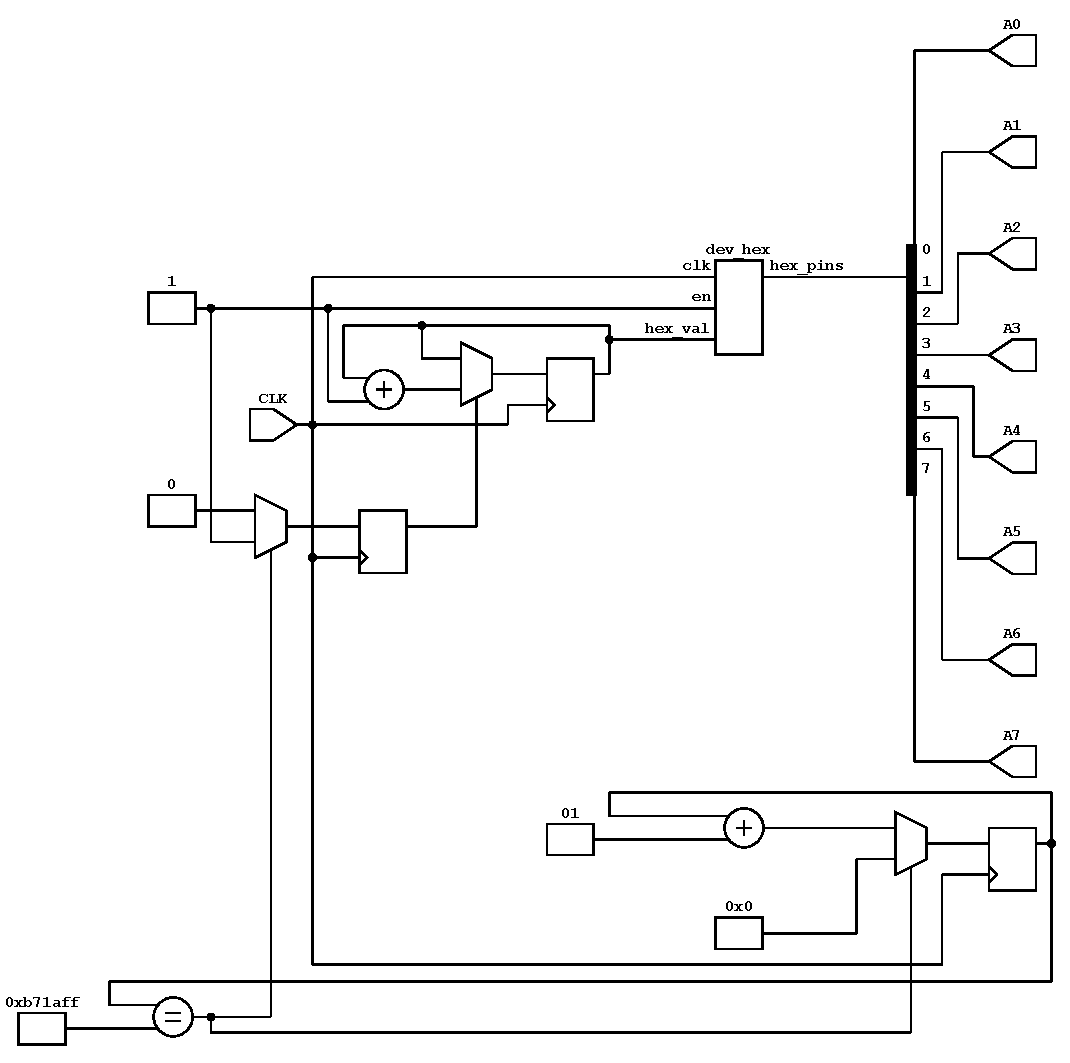
\includegraphics[width=0.8\linewidth]{figures/03_netlist.pdf}
\caption{The top module of step 03, drawn by \cc{make svg}. Bottom:
\cc{posEdgeCount} with its adder, the multiplexer that resets it and the
comparison with \cc{0xb71aff}${}= 11\,999\,999$. Middle left: \cc{tic}. Top:
\cc{hex_val} with its adder and the multiplexer that keeps the old value when
\cc{tic} is 0. The box \cc{dev_hex} is a module of its own.}
\label{fig:step03-netlist}
\end{figure}

All flip-flops in this design are clocked by the 12\,MHz clock \cc{CLK}. This
is the answer to the question at the end of Chapter~\ref{ch:step02}. We do not
build a slower clock; we build a signal that says ``now'' once per second, and
the register \cc{hex_val} takes over a new value only in those clock cycles.
Such a signal is called a \term{clock enable}. (One could also use the output
of a flip-flop as the clock of other flip-flops. But then the design has
several clocks whose edges are shifted against each other, and the tools can
no longer check the timing between them easily. We stay with one clock.)

\section{Vectors and Constants}
\label{sec:step03-vectors}

Here is the top module:

\svfile{03_hexdisplay/test.sv}

\textbf{Vectors.} \cc{logic [7:0] hex_val} declares eight signals
\cc{hex_val[7]}, \dots, \cc{hex_val[0]} under one name, a \term{vector}, like a
bus of eight wires in CircuitVerse. The range \cc{[7:0]} says that the bits are
numbered from 7 on the left down to 0 on the right. Whenever we compute with
a vector, it stands for the unsigned number
\[
  u(\mathit{hex\_val}) = \sum_{i=0}^{7} \mathit{hex\_val}_i \cdot 2^i ,
\]
so \cc{hex_val[7]} is the most significant bit. Parts of a vector are written
\cc{hex_val[3:0]} (the low four bits, a \term{nibble}) or \cc{hex_val[7:4]}
(the high nibble). In \cc{dev_hex} you will also see \cc{counter[2 +: 3]}:
three bits, starting at bit 2 and counting upward, which is the same as
\cc{counter[4:2]}. None of this is hardware; it only names wires.

\textbf{Concatenation.} Braces put signals side by side into one vector, the
first one on the left (most significant). Line 14,
\begin{lstlisting}
assign {A7, A6, A5, A4, A3, A2, A1, A0} = hex_pins;
\end{lstlisting}
has a concatenation on the left side: it splits the vector \cc{hex_pins} into
its bits, \cc{A7} gets \cc{hex_pins[7]} and \cc{A0} gets \cc{hex_pins[0]}. The
ports have to be single bits with the names from \cc{icebreaker.pcf}, where
\cc{A0} to \cc{A7} are the pins of PMOD 1A with the display. Inside, we
prefer to work with a vector. On the right side, as in \cc{dev_hex},
\cc{{digit_sel, seg_pins}} joins a bit and a 7-bit vector into 8 bits.

\textbf{Literals with a size.} A constant can be given with its number of bits
and its base: \cc{8'h0} is the number 0 as 8 bits in hexadecimal notation,
\cc{1'b1} a single 1 bit, \cc{7'b1000000} seven bits in binary, \cc{4'hA} the
four bits \cc{1010}. The format is \emph{width}\,\cc{'}\,\emph{base}\,\emph{digits}
with base \cc{b}, \cc{d} or \cc{h}. Underscores are ignored and only help
reading: \cc{12_000_000}. A number without a size, like \cc{1} or \cc{0}, has
32 bits. In hardware a constant is a wire tied to 0 or 1.

\textbf{\cc{localparam} names a constant.} \cc{localparam CLK_FREQ = 12_000_000;}
gives the number a name. It is not a signal and creates no hardware: wherever
\cc{CLK_FREQ} appears, the tools use the number. Even \cc{CLK_FREQ - 1} in
line 26 is computed by the tools, not by a subtractor: in
Figure~\ref{fig:step03-netlist} it is the constant \cc{0xb71aff} at the
comparator.

\textbf{\cc{integer}} is a 32-bit signed variable, an older type from Verilog.
In hardware, \cc{posEdgeCount} becomes 32 flip-flops, as we will see.

\textbf{Declaration with a value.} \cc{logic tic = 0;} declares \cc{tic} and
gives it the value 0 at the start. This is the same as an \cc{initial} block
(Chapter~\ref{ch:step02}): the power-up value of the flip-flops. The same
holds for \cc{posEdgeCount} and \cc{hex_val}. Verilator again reminds us that
these signals are also written in an \cc{always_ff} block:
\begin{terminal}
%Warning-PROCASSINIT: test.sv:21:17: Procedural assignment to declaration with
initial value: 'tic'
\end{terminal}
For us this is intended, as with \cc{MULTIDRIVEN} in Chapter~\ref{ch:step02}.

\section{Counters}
\label{sec:step03-counter}

\textbf{A counter is a register and an adder.} The block of lines 35--39 says:
at a rising edge of \cc{CLK}, \cc{hex_val} takes over \cc{hex_val + 1} if
\cc{tic} is 1. Read it as a circuit: an 8-bit register (eight flip-flops)
whose output goes through an adder that adds 1, and whose input is the output
of that adder. This is the counter you built in CircuitVerse.

The adder has eight output bits, so it computes modulo $2^8$:
\[
  u(\mathit{hex\_val}') = \bigl(u(\mathit{hex\_val}) + 1\bigr) \bmod 2^8 ,
\]
and after \cc{8'hff} comes \cc{8'h00}. (Strictly, \cc{hex_val + 1} has 32 bits,
because the literal \cc{1} has 32 bits. Assigning it to the 8-bit \cc{hex_val}
drops the upper 24 bits, and the result is the same.)

\textbf{\cc{if} in \cc{always_ff} is a multiplexer.} What happens if \cc{tic}
is 0? The block does not say, and for a flip-flop that means: it keeps its
value. So in front of the data input of the register there is a multiplexer
(Figure~\ref{fig:step03-netlist}, top) that selects between the new value
\cc{hex_val + 1} and the old value \cc{hex_val}, and \cc{tic} is its select
input. A register whose next value is either a new value or its old one,
depending on a signal, is a register with an \term{enable}, and the iCE40 has
a flip-flop for exactly this, \cc{SB_DFFE}. Mathematically,
\[
  \mathit{hex\_val}' =
  \begin{cases}
    \mathit{hex\_val} + 1, & \text{if } \mathit{tic} = 1,\\
    \mathit{hex\_val}, & \text{otherwise.}
  \end{cases}
\]

\textbf{Several assignments: the last one wins.} The block of lines 23--30
assigns \cc{posEdgeCount} and \cc{tic} twice:
\begin{lstlisting}
posEdgeCount <= posEdgeCount + 1;
tic <= 0;
if (posEdgeCount == CLK_FREQ - 1) begin
    posEdgeCount <= 0;
    tic <= 1;
end
\end{lstlisting}
The rule is: of all assignments to a signal in a block that apply, the last
one counts. So \cc{posEdgeCount} becomes 0 if it equals \cc{CLK_FREQ - 1}, and
\cc{posEdgeCount + 1} otherwise. And \cc{tic} becomes 1 in that case and 0
otherwise, in short $\mathit{tic}' = (u(\mathit{posEdgeCount}) =
11\,999\,999)$. This is a description of next-state functions, not a sequence
of steps: the comparison \cc{==} is a comparator circuit, the \cc{if} is a
multiplexer behind the adder, and both flip-flops take over their new values
at the same edge, as in Chapter~\ref{ch:step02}.

So \cc{posEdgeCount} runs through $0, 1, \dots, 11\,999\,999, 0, 1, \dots$,
twelve million values, and \cc{tic} is 1 in the clock cycle right after
\cc{posEdgeCount} was $11\,999\,999$: once every $12\,000\,000$ cycles,
exactly once per second. A counter that produces such a pulse once every $N$ cycles is
a \term{clock divider}, even though no new clock comes out of it.

\begin{exercise}
\label{ex:step03-period}
An earlier version of \cc{test.sv} compared with \cc{CLK_FREQ} instead of
\cc{CLK_FREQ - 1}. How many clock cycles lay between two cycles in which
\cc{tic} was 1, and how long was the ``second'' of that design? Would you
have noticed on the board?
\end{exercise}

\section{Using a Module: dev\_hex}
\label{sec:step03-instance}

Lines 41--46 place the display driver into our design:
\begin{lstlisting}
dev_hex dev_hex0 (
    .clk(CLK),
    .en(1'b1),
    .hex_val(hex_val),
    .hex_pins(hex_pins)
);
\end{lstlisting}
This is an \term{instance} of the module \cc{dev_hex}: a copy of the circuit
described in \cc{dev_hex.sv}, named \cc{dev_hex0}, with its ports connected to
our signals. In CircuitVerse terms, we place a subcircuit and wire it up.
\cc{.clk(CLK)} connects the port \cc{clk} of the instance to our signal
\cc{CLK}. Connecting by name is safer than by position, and we always do it.
The port \cc{en} is connected to the constant 1: the display is always on. We
could place several instances of the same module, each with its own name and
its own flip-flops.

The Makefile passes all \cc{.sv} files of the directory to the tools
(\cc{SV_FILES := $(wildcard *.sv)}), so \cc{dev_hex.sv} is found without
further ado; which module is the top module is given by \cc{-top test}.

\section{Driving the 7-Segment Display}
\label{sec:step03-display}

Each digit of the display consists of seven LED segments, called $a$ to $g$
(Figure~\ref{fig:step03-segments}). The module has only eight signal lines,
not $2 \cdot 7$: the seven segment lines are shared by both digits, and the
eighth line selects which of the two digits is switched on. So at any moment
at most one digit shows something. To show two digits, the driver alternates
between them, so fast that the eye sees both at once. This is called
\term{multiplexing} a display.

\begin{figure}[ht]
\centering
\begin{tikzpicture}[scale=0.55,
    seg/.style={line width=4pt,line cap=round,draw=red!75!black},
    lbl/.style={font=\small}]
  % one digit, segment a at the top, g in the middle
  \draw[seg] (0.3,4) -- (1.7,4);   \node[lbl,above] at (1,4.2) {$a$};
  \draw[seg] (2,3.7) -- (2,2.3);   \node[lbl,right] at (2.2,3) {$b$};
  \draw[seg] (2,1.7) -- (2,0.3);   \node[lbl,right] at (2.2,1) {$c$};
  \draw[seg] (0.3,0) -- (1.7,0);   \node[lbl,below] at (1,-0.2) {$d$};
  \draw[seg] (0,1.7) -- (0,0.3);   \node[lbl,left] at (-0.2,1) {$e$};
  \draw[seg] (0,3.7) -- (0,2.3);   \node[lbl,left] at (-0.2,3) {$f$};
  \draw[seg] (0.3,2) -- (1.7,2);   \node[lbl,above] at (1,2.1) {$g$};
  \node[anchor=west,align=left,font=\small] at (4.5,2) {%
    \begin{tabular}{@{}l@{}}
    \cc{seg_pins[0]} = $a$, \dots, \cc{seg_pins[6]} = $g$\\[2pt]
    0 = segment on, 1 = segment off\\[2pt]
    \cc{hex_pins} = \cc{{digit_sel, seg_pins}}, pins \cc{A7}, \dots, \cc{A0}
    \end{tabular}};
\end{tikzpicture}
\caption{The segments of one digit, and how \cc{dev_hex} encodes them.}
\label{fig:step03-segments}
\end{figure}

\subsection*{The segments: a truth table}

Which segments show a hexadecimal digit is a function
$\{0,1\}^4 \to \{0,1\}^7$, and the last block of \cc{dev_hex.sv} is its truth
table:

\svpart{firstline=58,lastline=77}{03_hexdisplay/dev_hex.sv}

\textbf{\cc{case} selects by value.} The \cc{case} statement compares
\cc{digit} with each of the values on the left and applies the assignment of
the matching one. In an \cc{always_comb} block it describes combinational
logic, here literally a table with 16 rows and 7 output columns. The bits are
written from \cc{segments[6]} ($g$) on the left to \cc{segments[0]} ($a$) on
the right, and a 0 switches a segment on. For example, \cc{4'h1} gives
\cc{1111001}: only $b$ and $c$ are on, the two segments on the right, which
form a ``1''. And \cc{4'h8} gives \cc{0000000}, all segments on.

Every segment is a Boolean function of the four bits of \cc{digit}. A function
of four bits is exactly what one LUT computes (Section~\ref{sec:lut}), so the
whole table becomes seven LUTs, one per segment.

\begin{pitfall}
A \cc{case} in \cc{always_comb} must assign a value in \emph{every} case.
Here it does: all 16 values of a 4-bit \cc{digit} are listed. If a case were
missing, the output would have to keep its old value for that input, and a
combinational circuit cannot keep anything. The tools then build a
\term{latch}, a storage element without a clock, which is almost never what
you want. Assigning a default value first, as the block that computes
\cc{digit} does with \cc{digit = 0;}, avoids this. In \cc{always_ff}, by contrast, a missing assignment is fine:
the flip-flop keeps its value, as we saw with \cc{hex_val}.
\end{pitfall}

\subsection*{Multiplexing the two digits}

The rest of \cc{dev_hex} decides which digit is shown when:

\svpart{firstline=13,lastline=46}{03_hexdisplay/dev_hex.sv}

\textbf{A counter as a time base.} \cc{counter} is a 30-bit counter that is
incremented at every clock edge. Only its bits 4 to 2 are used: line 17
connects them to \cc{display_state}. They change every 4 clock cycles and run through
$0, 1, \dots, 7$ once every 32 cycles, which is the 375\,kHz of the comment
($12\,\text{MHz} / 32$). yosys notices that bits 5 to 29 are never used and
removes them, so only five flip-flops remain. (\cc{always @(posedge clk)} is
the older Verilog form of \cc{always_ff @ (posedge clk)}, and describes the same
flip-flops here.)

\textbf{Which nibble.} The next block is a multiplexer:

\svpart{firstline=48,lastline=56}{03_hexdisplay/dev_hex.sv}

In states 0 and 1, \cc{digit} is the low nibble \cc{hex_val[3:0]},
in states 4 and 5 the high nibble, otherwise 0.

\textbf{When.} The \cc{case} in the clocked block sets the registers
\cc{seg_pins} and \cc{digit_sel} depending on the state:
\begin{center}
\begin{tabular}{cll}
\toprule
\cc{display_state} & \cc{seg_pins} & \cc{digit_sel} \\
\midrule
0, 1 & segments of the low nibble & (keeps 1) \\
2 & all off (\cc{~0}) & \\
3 & & becomes 0 \\
4, 5 & segments of the high nibble & (keeps 0) \\
6 & all off & \\
7 & & becomes 1 \\
\bottomrule
\end{tabular}
\end{center}
(\cc{~0} inverts the 32-bit number 0, and the lower 7 bits of the result, all
ones, go into \cc{seg_pins}.) Figure~\ref{fig:step03-mux} shows one period.
While \cc{digit_sel} is 1 the display shows the low nibble, which must
therefore be the right digit; while it is 0, the high nibble on the left. The
select line changes only in states 3 and 7, while all segments are off. If it
changed while segments were on, the other digit would light up briefly with
the wrong pattern, a faint ``ghost''. Each digit is on for 8 of the 32 cycles,
the 25\,\% duty cycle of the comment.

\begin{figure}[ht]
\centering
\begin{tikzpicture}[x=3.3mm,y=6mm]
  \def\bus#1#2#3#4{% x1, x2, y, label
    \draw[signal] (#1+0.25,#3) -- (#2-0.25,#3) -- (#2,#3+0.3) -- (#2-0.25,#3+0.6)
      -- (#1+0.25,#3+0.6) -- (#1,#3+0.3) -- cycle;
    \node[font=\scriptsize] at ({(#1+#2)/2},#3+0.3) {#4};}
  \foreach \t in {0,4,...,32} {
    \draw[black!12] (\t,0.8) -- (\t,6.9);
    \node[below,font=\scriptsize] at (\t,0.8) {\t};
  }
  \foreach \name/\y in {CLK/6, display\_state/4.8, seg\_pins/3.6, digit\_sel/2.4, shown/1.2} {
    \node[anchor=east,font=\small\ttfamily] at (-0.3,\y+0.3) {\name};
  }
  \draw[clocksig] (0,6) \foreach \t in {0,...,33} { -- (\t,6) -- (\t,6.6) -- (\t+0.5,6.6) -- (\t+0.5,6) } -- (34,6);
  \foreach \s in {0,...,7} { \bus{4*\s}{4*\s+4}{4.8}{\s} }
  \bus{32}{34}{4.8}{0}
  \bus{0}{1}{3.6}{}
  \bus{1}{9}{3.6}{low nibble}
  \bus{9}{17}{3.6}{off}
  \bus{17}{25}{3.6}{high nibble}
  \bus{25}{33}{3.6}{off}
  \bus{33}{34}{3.6}{}
  \draw[signal] (0,3) -- (13,3) -- (13,2.4) -- (29,2.4) -- (29,3) -- (34,3);
  \bus{1}{9}{1.2}{right digit}
  \bus{17}{25}{1.2}{left digit}
  \node[note,anchor=north east] at (34,0.3) {clock cycles};
\end{tikzpicture}
\caption{One period of \cc{dev_hex}, 32 clock cycles. The registers
\cc{seg_pins} and \cc{digit_sel} change one clock edge after
\cc{display_state} enters a new state. ``shown'' is what lights up.}
\label{fig:step03-mux}
\end{figure}

\begin{pitfall}
Lines 16 and 17 declare \cc{display_state} and connect it with \cc{assign}.
An earlier version of \cc{dev_hex.sv} did both in one line,
\begin{lstlisting}
logic [2:0] display_state = counter[2 +: 3];
\end{lstlisting}
which looks like a connection, but by the rules of SystemVerilog it is a
declaration with an initial value, like \cc{logic tic = 0;} in \cc{test.sv}:
\cc{display_state} gets the value of \cc{counter[4:2]} once at the start and
keeps it. Verilator follows this rule: in \cc{make sim}, \cc{display_state}
stayed 0 while \cc{counter} counted, so the simulated display never switched
digits. yosys (via sv2v) treated the line as a connection, and on the board
the display worked. Simulation and hardware disagreed, and neither tool
warned. A declaration with a value is a power-up value; to connect, write
\cc{assign}. (The same version also used \cc{segments} in the clocked block
before declaring it further down. The tools accepted that, but a name should
be declared before it is used, as lines 19 and 20 do now.)
\end{pitfall}

\section{What yosys Makes of It}
\label{sec:step03-yosys}

yosys flattens the design: the instance \cc{dev_hex0} disappears as a box, and
its parts appear in the netlist with names that begin with \cc{dev_hex0.}. The
statistics:

\outputfile{step03_yosys_stat.txt}

There are now four kinds of flip-flops, all of them the flip-flop of a logic
cell with extra inputs: \cc{E} (enable), \cc{R} (reset to 0) and \cc{S} (set to
1). Reset and set are \emph{synchronous}, they act at the clock edge like the
data input. With the cell names from \cc{test.json} we can tell what each one
is:
\begin{center}
\begin{tabular}{rll}
\toprule
count & type & signals \\
\midrule
32 & \cc{SB_DFFSR}, with synchronous reset & \cc{posEdgeCount} \\
8 & \cc{SB_DFFE}, with enable & \cc{hex_val}, enabled by \cc{tic} \\
7 & \cc{SB_DFFESS}, with enable and synchronous set & \cc{seg_pins} \\
7 & \cc{SB_DFF}, plain & \cc{counter[4:0]}, \cc{digit_sel}, \cc{tic} \\
\bottomrule
\end{tabular}
\end{center}
The \cc{if} that resets \cc{posEdgeCount} became the \cc{R} input: when
the comparator says ``equal'', the flip-flops become 0 at the next edge. The
``all off'' of \cc{seg_pins} became the \cc{S} input. All 32 bits of the
\cc{integer} are there, although $12\,000\,000 < 2^{24}$ and the upper 8 bits
are always 0; yosys cannot know that (Exercise~\ref{ex:step03-width}).

\subsection*{Adders and the carry chain}

The 39 \cc{SB_CARRY} belong to the three adders: 30 to the 32-bit
\cc{posEdgeCount}, 6 to the 8-bit \cc{hex_val}, 3 to the 5 remaining bits of
\cc{counter}. Here is the netlist of the counter \cc{hex_val}, one building
block per line, with the generated net names abbreviated: \cc{d[i]} is the data
input of the flip-flop of bit $i$ and \cc{c[i]} the carry into bit $i$:

\outputfile{step03_counter_cells.txt}

Read it as a ripple-carry adder for $h + 1$, with $h$ = \cc{hex_val}. Adding
1 means: bit $i$ flips if all bits below it are 1. With the carry $c_i$ into
bit $i$,
\[
  c_0 = 1, \qquad
  d_i = h_i \xor c_i, \qquad
  c_{i+1} = h_i \wedge c_i .
\]
For bit 0 this is $d_0 = \neg h_0$, a LUT that inverts (\cc{LUT_INIT} 1 for
$h_0 = 0$), and the carry into bit 1 is $h_0$ itself. For every other bit, a
LUT computes $h_i \xor c_i$ (\cc{0110100110010110} is the XOR of all four
inputs, two of which are 0), and an \cc{SB_CARRY} computes the carry. An
\cc{SB_CARRY} computes the carry of a full adder, $I_0 I_1 \vee (I_0 \vee
I_1)\,\mathit{CI}$, which is $h_i \wedge c_i$ for $I_0 = 0$.

The \cc{SB_CARRY} is not a LUT. It is a small piece of fixed logic in every
logic cell, next to the LUT, with a direct wire to the logic cell above it in
the same column. These wires form the \term{carry chain}. nextpnr places the
bits of an adder in consecutive logic cells of one column, so that the carry
runs up the chain without using the general routing.

\section{What nextpnr Makes of It}
\label{sec:step03-pnr}

\outputfile{step03_pnr_util.txt}

75 logic cells. \cc{SB_GB} is one of the eight \term{global buffers}: the
clock reaches all flip-flops over a special network with little delay
difference between them, and nextpnr puts \cc{CLK} on it.

The slowest path now starts at \cc{posEdgeCount[0]} and runs along the carry
chain to the top bit:

\outputfile{step03_pnr_path.txt}

Each step along the chain takes 0.28\,ns, and the positions show the chain
climbing the column $x = 4$ from tile $(4,1)$ to tile $(4,4)$: eight logic
cells per tile, four tiles for 32 bits. 30 steps of 0.28\,ns are the largest
part of the 15.32\,ns. The maximal clock frequency, 65\,MHz, is still far
above our 12\,MHz. But we see a rule: the longer an adder, the slower the
design. In the ULM, with its 64-bit adder, this will matter.

\begin{exercise}
\label{ex:step03-width}
Declare \cc{posEdgeCount} as \cc{logic [23:0]} instead of \cc{integer}. Why
are 24 bits enough? Predict the changes in the statistics of yosys, then check
them, and look at the logic cells and the maximal frequency in the output of
nextpnr.
\end{exercise}

\section{Simulation}
\label{sec:step03-sim}

The testbench toggles the clock, 35 rising edges in all. That is enough to
see \cc{posEdgeCount} and \cc{counter} count in the waveform viewer, and to
see the display switch digits: after each rising edge, the testbench compares
the output \cc{A7}, which is \cc{digit_sel}, with its value one edge before,
and counts the changes. At the end it prints the count, and if \cc{digit_sel}
never changed, it ends with an error, so that \cc{make sim} fails. This is
exactly the check that would have caught the mistake of the pitfall above.
\cc{tic}, however, would need twelve million edges. For a simulation we make
the second shorter:

\begin{exercise}
\label{ex:step03-sim}
Set \cc{CLK_FREQ} to 2 and \cc{MAX_SIM_TIME} in \cc{tb_test.cpp} to 200, and
run \cc{make sim}. Predict at which clock edges \cc{tic} is 1 and when
\cc{hex_val} changes, and check it in the waveform viewer. Then look at
\cc{display_state}, \cc{digit_sel} and \cc{seg_pins}, and compare with
Figure~\ref{fig:step03-mux}.
\end{exercise}

(Remember to undo the change of \cc{CLK_FREQ} before you program the board.)

\section{What Is Next}

The board now shows a number, and we know how to make something happen at a
human pace with a 12\,MHz clock. The display driver \cc{dev_hex} stays with us
until the last step. What is still missing is input: in step 04, the number on
the display comes from the DIP switch, stored into a register at the press of
a button.

\solutions

\solution
With \cc{== CLK_FREQ}, \cc{posEdgeCount} ran through $0, 1, \dots,
12\,000\,000$ and then started again at 0. These are $12\,000\,001$ values, so
\cc{tic} was 1 every $12\,000\,001$ cycles, and the second was one clock
cycle, $83$\,ns, too long. On the board nobody notices: after a day, the
display is 7\,ms behind. A counter that starts at 0 and should produce a pulse
every $N$ cycles has to start again after $N - 1$; such off-by-one errors are
found by counting in a simulation, not by watching the board.

\solution
The counter never exceeds $11\,999\,999 < 2^{24} = 16\,777\,216$, so 24 bits
hold all its values. With \cc{logic [23:0]}, yosys reports 24 \cc{SB_DFFSR}
instead of 32, 31 \cc{SB_CARRY} instead of 39 (8 fewer bits of the adder),
and 58 \cc{SB_LUT4} instead of 69. nextpnr then needs 64 logic cells instead of
75, and the maximal frequency rises from 65\,MHz to about 76\,MHz, because the
carry chain is 8 steps shorter.

\solution
With \cc{CLK_FREQ} = 2, \cc{posEdgeCount} runs through 0, 1, so \cc{tic}
is 1 in every second clock cycle, and \cc{hex_val} is incremented at the edge
that ends such a cycle: 1, 2, 3, \dots\ at every second edge.
\cc{display_state} changes every 4 cycles, \cc{seg_pins} shows the segments
of the low nibble, all ones, the segments of the high nibble, all ones, and
\cc{digit_sel} becomes 0 and 1 in the middle of the ``off'' phases, as in
Figure~\ref{fig:step03-mux}. (Since \cc{hex_val} now changes every two
cycles, the segments shown in one phase are those of the value when the phase
began, and may change during the phase.)
